\section{设计概览}
\label{sec:overview}

\sys 是一个面向技能的编译与运行时系统。
它将安装时对技能进行特化的 AOT 编译器~\cite{aho2006compilers}
与解决执行时不确定性的运行时结合起来，
使技能能够跨异构目标端移植。
图~\ref{fig:overview} 展示了其架构。

\begin{figure}[t]
  \centering
  \setlength{\belowcaptionskip}{-10pt}
  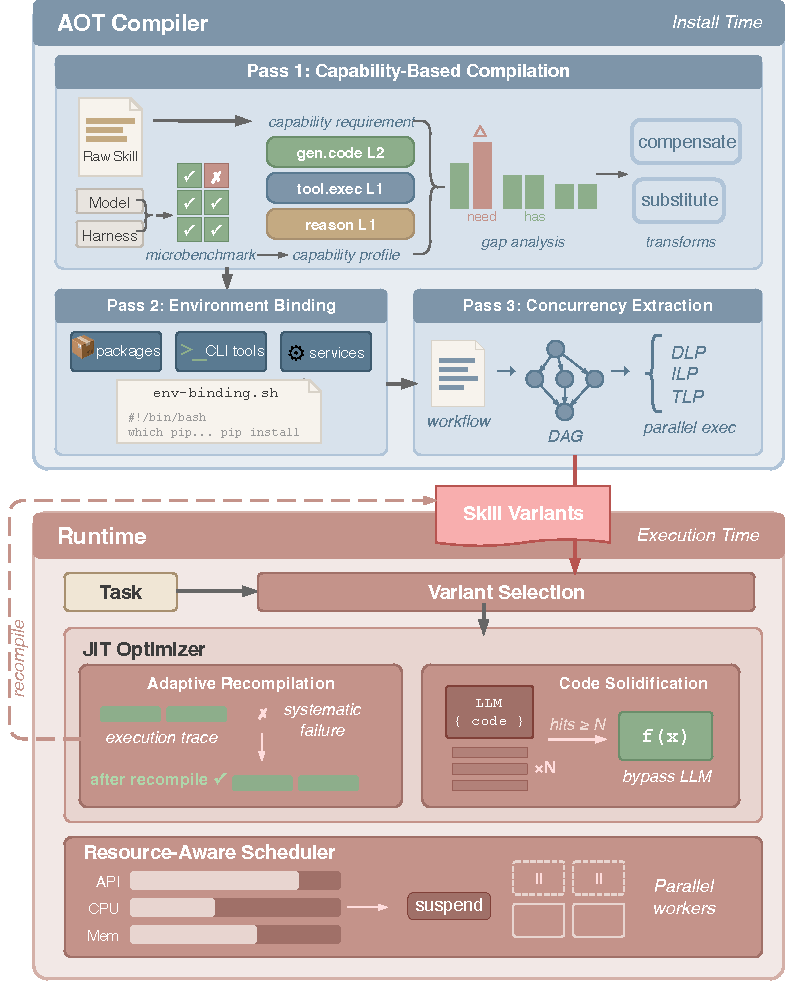
\includegraphics[width=\columnwidth]{figures/skillos_overview.pdf}
  \caption{\sys 架构。AOT 编译器在安装时经过三个编译阶段生成优化的技能变体；运行时则在执行期间负责变体选择、JIT 优化和资源感知调度。}
  \label{fig:overview}
\end{figure}

\heading{AOT 编译器。}
安装技能时，编译器针对目标环境分析该技能，并生成一个或多个优化后的
\emph{技能变体}。编译器执行三个彼此独立的阶段：
\emph{基于能力的编译}
（\S\ref{sec:compiler:cap}）通过使技能适配目标端可用的能力，
处理模型与代理框架的错配（P1--P2）。
\emph{环境绑定}
（\S\ref{sec:compiler:env}）通过具体化执行所需的依赖，
处理环境错配（P3）。
\emph{并发性提取}
（\S\ref{sec:compiler:par}）识别技能工作流中潜藏的并行性，并将其映射到目标代理框架。
编译后的变体会按目标端分别存储。

\heading{运行时与 JIT 优化器。}
任务到来时，运行时会选择为当前（模型，代理框架）组合编译的变体，
并通过标准的渐进式披露机制加载它。
随后，两个组件在常规执行之上发挥作用。
\emph{JIT 优化器}（\S\ref{sec:runtime:jit}）
跨调用监控执行结果，并在检测到 AOT 编译器未发现的能力缺口时触发重编译。
它还会把结构固定的代码模式编译成可执行函数，完全绕过 LLM 推理。
\emph{资源感知调度器}
（\S\ref{sec:runtime:sched}）连接编译时并行性标注与运行时资源可用性；
当需求超出容量时，它会节流或挂起并发子代理。
